
\definecolor{codegreen}{rgb}{0,0.6,0}
\definecolor{codegray}{rgb}{0.5,0.5,0.5}
\definecolor{codepurple}{rgb}{0.58,0,0.82}
\definecolor{backcolour}{rgb}{0.95,0.95,0.92}
 
\lstdefinestyle{mystyle}{
    backgroundcolor=\color{backcolour},   
    commentstyle=\color{codegreen},
    keywordstyle=\color{magenta},
    numberstyle=\tiny\color{codegray},
    stringstyle=\color{codepurple},
    basicstyle=\footnotesize,
    breakatwhitespace=false,         
    breaklines=true,                 
    captionpos=b,                    
    keepspaces=true,                 
    numbers=left,                    
    numbersep=5pt,                  
    showspaces=false,                
    showstringspaces=false,
    showtabs=false,                  
    tabsize=2
}
 
\lstset{style=mystyle}

\chapter{Developer Manual}
\settocdepth{chapter}
\label{appendix-developer-manual}

\section{Introduction}

This manual provides an overview of the initial steps needed to extend and further develop OKSE. The first sections are concerned with the set up of the development environment. The rest of explains the different parts of the system and how they may be extended. The system is open source, and licenced under the MIT licence\footnote{\url{http://opensource.org/licenses/MIT}}.

\section{Requirements and Setup}
The recommended setup, as noted below, is using IntelliJ IDEA\footnote{\url{https://www.jetbrains.com/idea/}} as the Java IDE. However, other IDEs that meet the requirements listed below, or a combination should suffice. 

\subsection{Java}
The minimum required major version of Java is 8, and it is recommend to use the latest minor release. Currently, Java 8 version 31 is the version used to compile the packaged version of OKSE.

\subsection{Apache Maven}
The project source code, tests and dependency management is structured with Apache Maven\footnote{\url{https://maven.apache.org}}. Maven is used to fetch dependencies, run tests and build the final jar files. The minimum major version of Maven is 3, and any minor version from 3.0.5 and up can be used. The version used for the current version of the system is 3.3.3.

It is worth mentioning that many of the popular Java IDE's has Maven support. Thus, its not required to install it separately.

\subsection{Recommended IDE}
The development team strongly recommends IntelliJ IDEA Ultimate\footnote{\url{https://www.jetbrains.com/idea/}} as the Integrated Development Environment. Note that the free Community edition should suffice, although the Ultimate edition has better support for frameworks like Spring and TestNG (test framework of choice), which is used for the web administration interface. Both Community and Ultimate edition comes bundled with Maven.

\subsubsection{IntelliJ IDEA setup}
As the user stands free to choose the IDE, the setup documentation will be fairly basic and based on IntelliJ IDEA.

Prerequisites: IntelliJ IDEA is installed, an Internet connection and the source code is stored locally.

\begin{enumerate}
\setlength{\itemsep}{0cm}%
    \item Open IntelliJ IDEA
    \item Click "Import Project" or File $\rightarrow$ "Import Project"
    \item Browse the file system and select the source code folder
    \item Choose "Import project from external model"
    \item Choose "Maven"
    \item Check "Import Maven projects automatically"
    \item Click Next
    \item no.ntnu.okse... should be selected, click Next
    \item Select 1.8 (if it is not available, click "+" and add it)
    \item Click Next
    \item Click Finish
\end{enumerate}

After the IntelliJ IDEA window is opened with the project, all the needed dependencies will be downloaded. After this is complete, the project setup is complete.

\subsection{Test Framework: TestNG}
The system has a lot of unit tests, written with the test framework TestNG\footnote{\url{http://testng.org/doc/index.html}}. Any new features and expansions of the system should be accompanied by unit tests. Please refer to the TestNG documentation\footnote{\url{http://testng.org/doc/documentation-main.html}} for information and documentation.

\section{Common Patterns Used}
\label{sec:common-patterns-used}

\subsection{Service oriented architecture}

Although there exists no formal definition or agreement upon what constitutes a service oriented architecture, some main principles are common. The OKSE message brokering system is implemented with some of these principles in mind. They include, but are not limited to:

\begin{itemize}
\item Service loose coupling: Minimize dependencies
\item Service abstraction: Hide logic from the outside world
\item Service re-usability: The DRY (Don't repeat yourself) principle
\item Service autonomy: Services have complete control over their own logic
\item Service encapsulation: Services incorporate other sub-components that were not service oriented, but serve as a part of the larger entity.
\end{itemize}

\subsection{Module pattern}

Software module pattern is a design pattern that emphasizes on organizing software components into modules. Some languages have this built into the language, but similar results can be accomplished through patterns. One way of creating modules is through the singleton pattern, described in the next section. OKSE implements several "tools" or "library" classes, which are considered software modules through their static references, and their manipulation of data from other sources.

\subsection{Singleton pattern}

The singleton pattern is a specialization of the module pattern. It is used to guarantee that an object cannot be instantiated more than once. Any further invocation would return the already instantiated object. This secures a single state for that particular component or module. In the case of the OKSE message brokering system, all services and protocol servers adhere to this pattern. This ensures that all references to a service point to the same instance.

This also makes it easier to reference the different services, as they are all referenced statically from their class. This means that it is not necessary to keep a local reference to the service in another class, or pass it as an argument to a certain method.

A practical example of how the singleton pattern is implemented in the OKSE core services and protocol servers, see sections \ref{sec:adding-new-protocols} and \ref{sec:adding-new-core-services}

\subsection{Reactor pattern}

In the OKSE system, all services and protocol servers are run in their own personal thread. To ensure a thread safe execution environment, inspiration was gathered from the reactor pattern. The reactor pattern generally receives events concurrently, and demultiplexes them synchronously, before dispatching to event handlers.

Although the OKSE system does not strictly implement separate dispatchers and event handlers, the basic idea stays the same. All singletons block on an internal task queue, awaiting new tasks (events) to be performed. The exact structure of these events and how they are consumed vary from service to service.

This approach allows different threads running client requests to concurrently perform tasks on the services without having to worry about concurrent modification errors.

\subsection{Observer pattern}

Due to the asynchronous nature of the services, listener support is implemented in most of them. This allows the service in question to invoke callback methods synchronously after a task has been completed. The more general use of the observer pattern is that all changes in internal state at the core service level, will also update registered listener components. This allows components such as the WSNSubscriptionManager to automatically synchronize its internal state when a change occurs in the OKSE SubscriptionService.

\section{Components}
\label{sec:developer_manual-components}
This section provides an overview of which steps are needed to extend the system with new services and protocols. For general system reference and the interaction of existing components, see chapter \ref{sec:architecture_and_implementation-implementation}.

\subsection{Application}
\label{subsec:developer_manual-components-application}

The \verb!Application.java! file that resides in the root of the project is the main invocation point when starting the OKSE application. The operations performed in this class are initializing the web admin console and the CoreService instance, which in turn boots up more services.

The most important thing to note regarding this main class, is that it is also the class in which further extensions should be registered. Extending the application with additional core services is done through registering them to the CoreService via the \\\verb!registerCoreService()! method.

Extending the application with additional protocol support is done through use of the \verb!addProtocolServers()! method of the CoreService instance.

The \verb!Application! class also exposes a static method for reading in configuration files. This method will also verify that the directory structure and necessary files exist. The \verb!readConfigurationFiles()! method does all this, and returns a \verb!Properties! object, which contains all the key-value pairs of the OKSE configuration file.

\subsection{Administration interface}
\label{subsec:administration_interface}

The OKSE administration console is built on the Spring framework, more exactly the spring-boot package\footnote{\url{https://spring.io/guides/gs/rest-service/}} with Thymeleaf-templates\footnote{\url{http://www.thymeleaf.org}}. The main aspects of the Web Admin component are its models, controllers, templates and front-end JavaScript. The administration interface is built in a modular way, to achieve loose coupling of modules. Each pane of the interface has its own controller and respective front-end JavaScript.  With this approach it is easy to extend the web interface.

\subsubsection{Back-end}

The back-end of OKSE works as a RESTful Web Service. As the back-end uses the Spring framework, the main architectural approach for the back-end is based on Spring’s approach for building RESTful web services. All HTTP-requests are handled by a dedicated controller. These controllers are easily identified by the \verb!@RestController! annotation. Each controller is responsible for handling all HTTP-requests on given routes defined by \verb!@RequestMapping! annotations. 

\subsubsection{Front-end}

The front-end of OKSE is the only component of the system that is directly accessible for graphical user interaction. It is responsible for making HTTP-requests to the back-end for manipulation and presentation of the state OKSE is currently in. See chapter \ref{subsec:architecture_and_implementation-implementation} for a more detailed description of the front-end architecture.

\subsection{Interacting with the MessageService}
\label{subsec:components-interacting_with_the_messageservice}

The MessageService is responsible for distributing messages to all the registered protocol servers. It provides a simple interface to put messages up for processing. The following code snippet shows how messages are created and distributed.

\begin{lstlisting}[language=Java, captionpos=b, caption=Distributing a message, frame=bt, showstringspaces=false]
    // Define a topic
    String topic = "no/ffi";
    // Create som content
    String msg = "some data";
    // Fetch a related publisher, null if none is relevant
    Publisher p = null;
    // Set the originating protocol, must be the same as
    // the protocolServerType field in the ProtocolServer class.
    String originProtocol = "WSNotification";
    
    // Create a Message object
    Message m = new Message(msg, topic, p, originProtocol);
    // Distribute the message
    MessageService.getInstance().distributeMessage(m);
\end{lstlisting}

The MessageService also allows requestors to retrieve the last message sent on a topic, regardless of originating protocol. This is done in the following fashion.

\begin{lstlisting}[language=Java, captionpos=b, caption=Retrieving latest message on a topic, frame=bt, showstringspaces=false]
    // Initialize the message variable
    Message m;
    // Fetch the latest message
    m = MessageService.getInstance().getLatestMessage("topic/subtopic");
    
    // Check if there was any message
    if (m != null) {
        /* Do something with the message */
    }
\end{lstlisting}

Another handy helper method is the ability to take a single message, and duplicate it to all the topics in a provided set of topics. Most of the time, strings are used to represent topics, for ease of use. Still, the actual topics are stored in Topic objects. This helper method uses Topic objects.

\begin{lstlisting}[language=Java, captionpos=b, caption=Duplicating message to multiple topics, frame=bt, showstringspaces=false]
    // Create a message
    Message m = new Message("<data>1</data>", "hq/test", null, "WSNotification");

    // For example, retrieve all Topics that are root nodes
    HashSet<Topic> topicSet = TopicService.getAllRootTopics();
    // Fetch an additional topic node
    Topic extraTopic = TopicService.getTopic("no/ffi");
    // Add it to the set
    topicSet.add(extraTopic);
    
    // Generate a list of messages destined to each of the
    // provided topics
    List<Message> generated = MessageService.getInstance()
        .generateMessageForAGivenTopicSet(m, topicSet);
        
    /* Do some action on the messages, for example... */
    generated.forEach(m -> MessageService.getInstance().distribute(m));
\end{lstlisting}

\subsection{Interacting with the TopicService}
\label{subsec:components-interacting_with_the_topicservice}

The TopicService is responsible for maintaining an overview of all topics that have been referenced at some time. It exposes a general API for adding and removing topics, as well as several methods for retrieving topics.

A Topic in itself is a part of a tree of nodes. It may have a parent, and it may have children. The TopicService keeps track of all these trees. For the implemented protocols in the OKSE system, none use this hierarchical nature. Still, they are represented in this way for future use.

In order to retrieve the canonical name of a topic, one uses the \verb!getFullTopicStrin! \verb!g()! method on a Topic object. This representation is what is expected in all parts of the OKSE system that accepts topics represented by strings.

The following code shows how to add a new topic to the system.

\begin{lstlisting}[language=Java, captionpos=b, caption=Adding a new topic, frame=bt, showstringspaces=false]
    // Add a new topic
    TopicService.getInstance().addTopic("no");
    
    // Add another topic
    TopicService.getInstance().addTopic("no/ffi/uav");
\end{lstlisting}

In the second \verb!addTopic! call, the TopicService will identify that the \verb!no! topic already exists. It will only generate the new topic nodes that are needed, link these together, and connect the branch to the already existing \verb!no! topic node. After the second \verb!addTopic! call, the \verb!no! topic node is reachable by traversing the tree from \verb!uav! by using the \verb!getPare! \verb!nt()! method of a topic node.

The following code snipped demonstrates how Topics are removed from the system.

\begin{lstlisting}[language=Java, captionpos=b, caption=Deleting a topic, frame=bt, showstringspaces=false]
    // Add some topics
    TopicService.getInstance().addTopic("no/ffi/uav");
    
    // Delete the intermediate node
    TopicService.getInstance().deleteTopic("no/ffi");
\end{lstlisting}

In this example, three topic nodes are created and linked together in a tree. When the \verb!no/ffi! node is deleted, its child \verb!uav! is also deleted. After the operation, only the \verb!no! topic node remains in the system.

The following examples show a selection of the service methods exposed by the TopicService.

\begin{lstlisting}[language=Java, captionpos=b, caption=Additional TopicService methods, frame=bt, showstringspaces=false]
    // Retrieve all leaf topic nodes
    HashSet<Topic> leafNodes = TopicService.getInstance().getAllLeafTopics();
    
    // Retrieve all root topic nodes
    HashSet<Topic> rootNodes = TopicService.getInstance().getAllRootTopics();
    
    // Get all topic nodes
    HashSet<Topic> allNodes = TopicService.getInstance().getAllTopics();
    
    // Check existance
    if (TopicService.getInstance().topicExists("no/ffi")) {
        /* Perform some action */
    }
\end{lstlisting}

It is worth mentioning that all the returned sets of topics are shallow clones of the originating data structure. This is to ensure that no accidental modification of the internal data structure is made.

\subsection{Interacting with the SubscriptionService}
\label{subsec:components-interacting_with_the_subscriptionservice}

The SubscriptionService is responsible for maintaining an overview of the currently registered subscribers and publishers. The SubscriptionService also periodically removes entities that have expired. Finally, the SubscriptionService is responsible for modifying the parameters connected to a specific entity.

The Subscriber object itself contains a selection of sets and attributes to service possible future needs. The following code sample illustrates some of these features. Publisher objects contain a subset of these features.

\begin{lstlisting}[language=Java, captionpos=b, caption=Properties of the Subscriber object, frame=bt, showstringspaces=false]
    // Host of the subscriber
    String host = "123.123.123.123";
    // Port of the subscriber
    Integer port = "52612";
    // The topic of the subscriber
    String topic = "no/ffi";
    // The originating protocol of the subscription
    String origProtocol = "AMQP";
    
    // Create the subscriber
    Subscriber sub = new Subscriber(host, port, topic, origProtocol);
    
    // Set an expiration time for the subscription
    // in milliseconds since UNIX epoch.
    sub.setTimeout(1234567890);
    
    // Set an attribute on the subscriber object
    // for some specific use
    sub.setAttribute("key", "value");
    
    // Get an attribute from the subscriber object
    String value = sub.getAttribute("key");
    if (value != null) {
        /* Perform some action */
    }
    
    // Store some sort of filter expression used by
    // the subscriber
    sub.addFilter("regex:^[a-zA-Z]+");
    sub.addFilter("//rootElement/*");
    
    /* These filters do not have any purpose but to 
    store the information for later retrieval, and
    list them in the administration interface */
    
    // Retrieve some general attributes from the subscriber
    sub.getHost();
    sub.getPort();
    sub.getTimeout();
    sub.getTopic();
    sub.getOriginProtocol();
    if (sub.shouldExpire()) { /* ... */ }
    if (sub.hasExpired()) { /* ... */ }
\end{lstlisting}

A subset of these fields and methods are also available for Publisher objects.

The following code sample illustrates how to add, update, and remove subscribers from the SubscriptionService.

\begin{lstlisting}[language=Java, captionpos=b, caption=Subscriber actions, frame=bt, showstringspaces=false]
    // Create a subscriber
    Subscriber sub = new Subscriber("10.0.0.1", "8080", "no/ffi", "AMQP");
    
    // Add it to the SubscriptionService
    SubscriptionService.getInstance().addSubscriber(sub);
    
    // Pause the subscription
    SubscriptionService.getInstance().pauseSubscriber(sub);
    
    if (sub.getAttribute("paused").equals("true") {
        /* true, subscriber is paused */
    } else {
        /* subscriber is not paused */
    }
    
    // Resume the subscription
    SubscriptionService.getInstance().resumeSubscriber(sub);
    
    // Renew the subscription
    Long newTerminationTime = 1234567890;
    SubscriptionService.getInstance().renewSubscriber(sub, newTerminationTime);
    
    // Remove it again
    SubscriptionService.getInstance().removeSubscriber(sub);
\end{lstlisting}

It is important to note that these methods only alter the internal state of the OKSE SubscriptionService and its Subscriber objects. It is up to the specific protocol implementations that have need of these features to use them where applicable.

The SubscriptionService also exposes a set of extra service methods that provide aggregation and selection capabilities. Some examples are listed in the code sample below.

\begin{lstlisting}[language=Java, captionpos=b, caption=Additional SubscriptionService methods, frame=bt, showstringspaces=false]
    // Cache the SubscriptionService reference for ease of access
    SubscriptionService ss = SubscriptionService.getInstance();
    
    // Get a subscriber by its unique ID
    Subscriber sub = ss.getSubscriberByID("a517...1c3f");
    
    // Get all subscribers or publishers for a topic
    HashSet<Subscriber> subscribers;
    HashSet<Publisher> publishers;
    subscribers = ss.getAllSubscribersForTopic("no/ffi");
    publishers = ss.getAllPublishersForTopic("no/ffi");
    
    // Get all subscribers and publishers
    HashSet<Subscriber> allSubscribers;
    HashSet<Publisher> allPublishers;
    allSubscribers = ss.getAllSubscribers();
    allPublishers = ss.getAllPublishers();
\end{lstlisting}

As with most collections returned by the services, sets are shallow copies of the internal structure in the service itself. This is done to prevent accidental modification of the internal structure.

When Subscribers or Publishers are created, modified or deleted, all registered listeners to the SubscriptionService are notified. They will receive either a SubscriptionChangeEvent or a PublisherChangeEvent. The following code sample illustrates how these events might be used.

\begin{lstlisting}[language=Java, captionpos=b, caption=Use of the SubscriptionService listener support, frame=bt, showstringspaces=false]
public class SomeListener implements SubscriptionChangeListener {
    public SomeListener() {
        SubscriptionService.getInstance().addSubscriptionChangeListener(this);
    }
    
    @Override
    public void subscriptionChanged(SubscriptionChangeEvent e) {
        SubscriptionChangeEvent.Type type = e.getType();
        Subscriber sub = e.getData();
        
        // If we for example are only interested in AMQP
        // related subscribers
        if (!sub.getOriginProtocol().equals("AMQP")) {
            return;
        }
        
        if (type == SubscriptionChangeEvent.Type.UNSUBSCRIBE) {
            /* Do some action for unsubscribe events */
            someLocalMapping.remove(sub);
        }
        /* else if (type == ...)
            Additional types are:
            
            SUBSCRIBE,
            PAUSE,
            RESUME,
            RENEW
        */
    }
}
\end{lstlisting}

\section{Adding new protocols}
\label{sec:adding-new-protocols}

The OKSE system was designed such that extending the system with additional protocols should be as easy as possible. Some boilerplate code is still needed to have a minimum foundation on which the protocol server is intended to run.

To add a new protocol to the OKSE system, the first step is to extend the \verb!AbstractPr! \verb!otocolServer! class. This will prompt the developer to implement a set of methods needed in a protocol server. Additionally, some extra static methods are needed for implementing it as a singleton.

Below is an example of the structure of a class extending from the \verb!AbstractProtoc! \verb!olServer! class.

\begin{lstlisting}[language=Java, captionpos=b, caption=Adding a new protocol, frame=bt, showstringspaces=false]
public class NewProtocolServer extends AbstractProtocolServer {

    // Generic statics
    private static Logger log;
    private static NewProtocolServer _singleton;
    private static Thread _serverThread;
    private static boolean _invoked;
    
    // Internal defaults
    private static final String DEFAULT_HOST = "0.0.0.0";
    private static final Integer DEFAULT_PORT = 1337;
    
    // Custom fields
    
    // Private constructor
    private NewProtocolServer(String host, Integer port) {
        init(host, port);
    }
    
    // Private init method
    private init(String host, Integer port) {
        // Host and port
        if (host == null) this.host = DEFAULT_HOST;
        else this.host = host;
        if (port == null) this.port = DEFAULT_PORT;
        else this.port = port;
        
        // Init the logger
        log = Logger.getLogger(NewProtocolServer.class.getName());
        
        // Protocol server type
        protocolServerType = "NewProtocol";
        
        // Update invoke flag
        _invoked = true;
    }
    
    // Public singleton object factory
    public static NewProtocolServer getInstance() {
        if (!_invoked) {
            String configHost = null;
            Integer configPort = null;
            
            /* Read from config file if exists... */
            
            _singleton = new NewProtocolServer(configHost, configPort);
        }
        
        return _singleton;
    }
    
    // Public boot method
    public void boot() {
        if (!_running) {
            _running = true;
            
            // Instantiate necessary objects
            // Start necessary support modules etc
            
            // Set up server thread
            _serverThread = new Thread(() -> this.run());
            _serverThread.setName(protocolServerType);
            _serverThread.start();
        }
    }
    
    // Public run method
    public void run() {
        while (_running) {
            // Main run loop that does what it is supposed to do.
            // Blocking on a queue, or awaiting connections etc
        }
    }
    
    // Stop method
    public void stopServer() {
        _running = false;
        _invoked = false;
        /*
            Stop server thread in here
                                        */
        _serverThread = null;
        _singleton = null;
    }
    
    // Get protocol type
    public String getProtocolServerType() {
        return this.protocolServerType;
    }
    
    // Send message method that is called from MessageService
    public void sendMessage(Message msg) {
        // Check that the message came from another protocol
        if (!msg.getOriginProtocol.equals(protocolServerType) {
            // Perform needed actions to send msg here
        }
    }
}
\end{lstlisting}

The only thing needed to include the new protocol in the OKSE system is to add it in the \verb!Application! class, through the \verb!CoreService!.

\begin{lstlisting}[language=Java, captionpos=b, caption=Registering a new protocol, frame=bt, showstringspaces=false]
        // Initialize main system components
        webserver = new Server();
        cs = CoreService.getInstance();

        /* ... */

        /* REGISTER PROTOCOL SERVERS HERE */
        cs.addProtocolServer(WSNotificationServer.getInstance());
        cs.addProtocolServer(AMQProtocolServer.getInstance());
        cs.addProtocolServer(NewProtocolServer.getInstance());
\end{lstlisting}

\section{Adding new core services}
\label{sec:adding-new-core-services}

The OKSE system was designed such that extending the system with additional core services should be as easy as possible. Some boilerplate code is still needed to have a minimum foundation on which the core service is intended to run.

To add a new core service to the OKSE system, the first step is to extend the \verb!Abstract! \verb!CoreService! class. This will prompt the developer to implement a set of methods needed in a core service. Additionally, some extra static methods are needed for implementing it as a singleton.

Below is an example implementation of a new core service, which extends the \verb!Abstra! \verb!ctCoreService! class. No clear purpose is defined for this service other than for the intent of clarifying the structure.

\begin{lstlisting}[language=Java, captionpos=b, caption=Creating a new core service, frame=bt, showstringspaces=false]
public class NewService extends AbstractCoreService {

    // Generic statics
    private static NewService _singleton;
    private static Thread _serviceThread;
    private static boolean _invoked;
    
    // Event queue
    private LinkedBlockingQueue<SomeEvent> queue;
    
    // Custom fields
    Properties config;
    
    // Protected constructor (for unit test subclassing purposes)
    protected NewService() {
        // Pass the classname to super to init the logger
        super(NewService.class.getName());
        if (_invoked) throw new IllegalStateException("Already invoked");
        init();
    }
    
    // Initialization helper method
    private init() {
        queue = new LinkedBlockingQueue<>();
        config = Application.readConfigurationFiles();
        _invoked = true;
    }
    
    // Static object factory for singleton
    public static NewService getInstance() {
        if (!_invoked) _singleton = new NewService();
        return _singleton;
    }
    
    // Public boot method
    public void boot() {
        if (!_running) {
            log.info("Booting NewService");
            _serviceThread = new Thread(() -> this.run());
            _serviceThread.setName("NewService");
            _serviceThread.start();
        }
    }
    
    // Public run method
    public void run() {
        _running = true;
        while (_running) {
            try {
                Event event = queue.take();
                /* Handle event here... */
                
            } catch (InterruptedException e) {
                log.error("Interrupted during event queue fetch");
            }
        }
        
        log.info("NewService stopped");
    }
    
    // Stop method
    public void stop() {
        _running = false;
        /* Stop serviceThread here */
        
        /* An example is to send a no-op event to the queue */
        _serverThread = null;
        _singleton = null;
        _invoked = false;
    }
    
    // Register listener support
    public void registerListenerSupport() {
        /*  Add all commands to register this new service
            as a listener to other services here
            as it will be called after all services
            are booted.
        */
    }
}
\end{lstlisting}

The only thing needed to include the service in the OKSE system is to register it in the \verb!Application! class, through the \verb!CoreService!.

\begin{lstlisting}[language=Java, captionpos=b, caption=Registering a new service, frame=bt, showstringspaces=false]
        // Initialize main system components
        webserver = new Server();
        cs = CoreService.getInstance();

        /* REGISTER CORE SERVICES HERE */
        cs.registerService(TopicService.getInstance());
        cs.registerService(MessageService.getInstance());
        cs.registerService(SubscriptionService.getInstance());
        cs.registerService(NewService.getInstance());

        /* ... */
\end{lstlisting}

\section{Extending the administration interface}
\label{sec:adding-new-panes}

This section describes how the administration interface might be extended with new content and functionality. Figure \ref{fig:spring} visualizes how the system handles events and exposes information to the users. The key concepts to notice here are the AJAX-requests and the controllers. On an event, whether it is a page auto update or a button-click, the request URL is accessed by the AJAX-request. Springs dispatcher maps the URL and forwards it to the correct controller. This controller interacts with OKSEs services and returns a response.

\begin{itemize}
    \item\textbf{Dispatcher} -  This is the class that is exposed to the user. It forwards request URLs to the mapping handler to reach the correct controller. It then calls the controller responsible for the request. Finally it returns the response to the user. 
    \item\textbf{Mapping handler} - This class maps the request URL to the controller responsible for the request, and returns it to the dispatcher. 
    \item\textbf{Controller} - This is the class responsible for executing tasks and getting information from the message broker. It returns a JSON response \footnote{\url{http://json.org}} string to the dispatcher.  
\end{itemize}

\clearpage

\begin{center}
  \begin{figure}[ht!]
    \makebox[\textwidth]{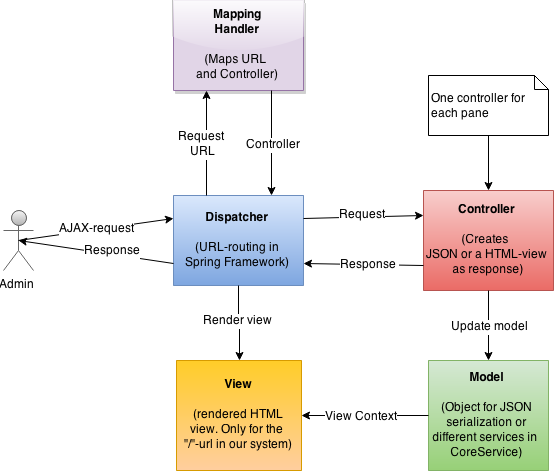
\includegraphics[width=0.8\textwidth]{fig/spring.png}}
    \caption{REST-API structure}
    \label{fig:spring}
  \end{figure}
\end{center}

The following steps explains how to actually extend the application. In addition, the following steps provides a guide to Thymeleaf templates, Spring, JavaScript and jQuery. 

\begin{itemize}
\setlength{\itemsep}{0cm}%
\item Thymeleaf - see \url{http://www.thymeleaf.org/documentation.html}
\item Spring framework - see \url{https://spring.io/guides/gs/rest-service/}
\item jQuery - see \url{http://jqfundamentals.com}
\item JavaScript - see \url{https://developer.mozilla.org/en-US/docs/Web/JavaScript/A_re-introduction_to_JavaScript}
\end{itemize}

\subsection{Administration interface structure}

All files for the administration interface are located in three main folders, \verb!static/js!, \verb!templates! and \verb!web!. See figure \ref{fig:oac-folder-hierarchy} for a detailed overview. To extend the application, the existing files can be copied or new ones created based on the skeleton provided in section \ref{subsubsec:skeletons}. The files that needs to be copied or created are:

\begin{itemize}
\item HTML template files in \verb!src/resources/templates/!
\item JavaScript files in \verb!src/resources/static/js/!
\item Spring controllers in \verb!src/no/ntnu/okse/web/controller/! 
\end{itemize}

\begin{center}
  \begin{figure}[ht!]
    \makebox[\textwidth]{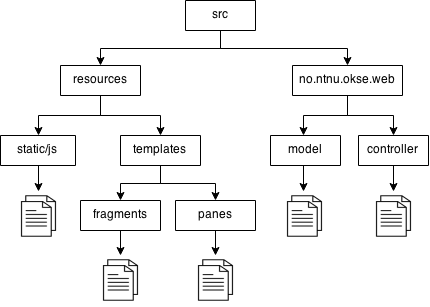
\includegraphics[scale=0.4]{fig/oacFolders.png}}
    \caption{Folder hierarchy for the administration interface}
    \label{fig:oac-folder-hierarchy}
  \end{figure}
\end{center}

\noindent OKSE contains of seven JavaScript modules: 

\begin{description}
    \item[main.js] \hfill \\ Responsible for the "Main"-pane. This module also contains all logic for setting the update interval all panes. Additionally, this is the location of the AJAX-module. 
    \item[topics.js] \hfill \\ Responsible for the "Topics"-pane. This module contains all logic regarding topics, and includes refreshing the table containing all topics. 
    \item[subscribers.js] \hfill \\ Responsible for the "Subscribers"-pane. This module contains all logic regarding subscribers. which includes, but are not limited to, refreshing the table containing all subscribers. 
    \item[stats.js] \hfill \\ Responsible for the "Statistics"-pane. This module contains all logic for refreshing the statistics from OKSE.
    \item[logs.js] \hfill \\ Responsible for the "Logs"-pane. This module requests the given log from OKSE and visualizes it.
    \item[config.js] \hfill \\ Responsible for the "Configuration"-pane. This module is responsible for the configuration of OKSE. This includes the possibility to add topic mappings. 
    \item[paginator.js] \hfill \\ This module controls all logic regarding the paginator that appears when the topic/subscriber tables exceed 25 elements. 
    \item[okseDebug.js] \hfill \\ This is a jQuery-plugin that appends a logger to the document.
\end{description}



\subsubsection{Skeletons}
\label{subsubsec:skeletons}

Below is a skeleton for adding a new REST controller. The same applies for normal controllers, with the \verb!@RestController! annotation changed to \verb!@Controller!. When using this annotation, Spring will automatically find the controller on boot, and add the mapping to the dispatcher. 

\begin{lstlisting}[language=Java, captionpos=b, caption=Skeleton for a REST-controller, frame=bt, showstringspaces=false]
@RestController
@RequestMapping(value = "/api/MYPANE") // Base URL
public class TestController() {
    
    private static final String TEST_URL = "/get/all";
    
    @RequestMapping(value = TEST_URL, method = RequestMethod.GET)
    public @ResponseBody void getAllInfo() {
        return "This is a test";
    }
    
}
\end{lstlisting}

Below is a skeleton for adding a new JavaScript module to the web page for displaying information from a controller. This only shows briefly how one would start to create new modules. To add the JS-file to the administration interface on rendering, append \verb!<script th:src="/js/<MODULE>.js"></script>! to the \verb!th:block! identified with "scripts" in the \verb!indexLoggedIn.html! template. \\ 

\begin{lstlisting}[language=Java, captionpos=b, caption=Skeleton for a JavaScript module, frame=bt, showstringspaces=false]
var MYPANE = (function($) { 

    var initateModule = function() {
    
    }

    return {
        init = intiateModule
    }

})(jQuery)
\end{lstlisting}

\begin{lstlisting}[language=HTML, captionpos=b, caption=Skeleton for a Thymeleaf-template, frame=bt, showstringspaces=false]
<html xmlns:th="http://www.thymeleaf.org"
      xmlns:layout="http://www.ultraq.net.nz/web/thymeleaf/
      layout"
      xmlns:sec="http://www.thymeleaf.org/thymeleaf-extras
      -springsecurity3"
      layout:decorator="layout">
<head>
</head>
<body>
<th:block layout:fragment="MYPANE">
<div class="tab-pane" id="MYPANE">
...
</div>
</th:block>
</body>
</html>
\end{lstlisting}

When adding a new pane it is important to register the panes corresponding JavaScript module in the \verb!main.js! file. This is done by appending a \verb!switch-case! for your pane. It is also important to register the panes template in \verb!indexLoggedIn.html!

\section{AMQP Send and Receive}
Along with the source code, two simple test classes for AMQP are bundled. One that implements a receiver and one that implements a sender. The classes are used for amqprecv.jar and amqpsender.jar files that can be used to test the broker as mentioned in \ref{subsec:test_clients-amqp_receive} and \ref{subsec:test_clients-amqp_send}. The example classes are located in the folder \verb!src/main/java/no/ntnu/! \verb!okse/examples/amqp! starting at the root of the project.

Both classes has Apache Qpid Proton as a dependency and it is recommended that they are used together with Maven to fetch the needed dependencies.

In the following sections, a walk-through of the most important parts of the implementation are provided. To get a deeper understanding of the implementation, the Qpid documentation\footnote{\url{http://qpid.apache.org/releases/qpid-proton-0.9.1/proton/java/api/index.html}} should be consulted.

\subsection{AMQPSender}
The example below implements the needed code to send a message on a topic to an existing AMQP 1.0 server.

\begin{lstlisting}[language=Java, captionpos=b, caption=Example use of Messenger to subscribe, frame=bt, showstringspaces=false,label={lst:AMQPSender}]
// variables
String address = "amqp://localhost:5672/example"
String body = "exampleMessage";
String subject = "exampleSubject";

Messenger mng = Messenger.Factory.create();
mng.start();
Message msg = Message.Factory.create();
msg.setAddress(address);

if (subject != null) msg.setSubject(subject);
msg.setBody(new AmqpValue(body));
mng.put(msg);
mng.send();
mng.stop();
\end{lstlisting}

\begin{description}
\item[1-3] \hfill \\ The first three lines declare variables, the server, port and topic. The second and third declares the message and the subject.
\item[6-7] \hfill \\ Lines 6 and 7 creates a message and starts it. The messenger is the client software that actually connects to the server.
\item[8-9] \hfill \\ Lines 8 and 9 creates an empty message and sets the address.
\item[12-13] \hfill \\ Lines 12 and 13 finishes the message and gives it to the manager.
\item[14] \hfill \\ Finally, line 14 will send the message to the given address.
\end{description}

\subsection{AMQPReceiver}
The example found below implements the needed code to subscribe to an existing AMQP 1.0 server.


\begin{lstlisting}[language=Java, captionpos=b, caption=Example use of Messenger to subscribe, frame=bt, showstringspaces=false,label={lst:AMQPReceiver}]
// variables
String address = "amqp://localhost:5672/example"
int maxMessages = 200;

Messenger mng = Messenger.Factory.create();
mng.start();
mng.subscribe(address);

int messages = 0;
boolean done = false;
while (!done) {
    mng.recv();
    while (mng.incoming() > 0) {
        Message msg = mng.get();
        ++ct;
        System.out.println(msg);
        if (maxMessages > 0 && messages >= maxMessages) {
            done = true;
            break;
        }
    }
}
mng.stop();
\end{lstlisting}

\begin{description}
\item[1-2] \hfill \\ The first two lines describe the declaration of variables. The first one is the AMQP server, the next is the amount of messages this particular implementation should accept before stopping.

\item[5-7] \hfill \\ Lines 5 to 7 creates an instance of the messenger, starts it and subscribes to the address defined earlier. Except for receiving the actual messages, this is basically what must be implemented to actually connect to a server.

\item[12] \hfill \\ Line 12 tells the messenger to start receiving from the server. 
\item[13-14] \hfill \\ Line 13 to 14 receive messages and creates messages as long as there are any to receive.

\item[15] \hfill The last lines check if the receive limit is met and stops the program if it is.
\end{description}

\clearpage